\documentclass[
    a0paper,
    portrait,
%    fontscale=0.05,
%    margin=1.7cm
]{baposter}

\usepackage{astro-poster}

\begin{document}

\begin{poster}{
  background=plain,
  bgColorOne=white,
  headerheight=0.11\textheight,
  columns=3,
  headershade=plain,
  headerColorOne=applegreen,
  boxColorOne=white,
  headershape=smallrounded,
  textborder=roundedsmall,
  linewidth=0.4pt,
  borderColor=bordergreen,
  headerborder=open,
  headerfont=\large\bf,
  boxpadding=2.2mm
}{QR
    
\includegraphics[width=0.60\headerheight]{fig/QR.pdf}
}{ \huge
    Cepheid pulsation mode identification via \\ unsupervised machine learning
}{
    \normalsize \vspace{2mm}
    Santiago Henao Castellanos,
    Alejandro García Varela \\ \vspace{1mm}
    \texttt{s.henao10@uniandes.edu.co}, 
    \texttt{josegarc@uniandes.edu.co}
    
    Physics department, Universidad de los Andes, Bogotá, Colombia \\ 
    
}{
    
\includegraphics[width=1.5\headerheight]{fig/logo-uniandes.pdf}
}

\begin{posterbox}[name=intro,column=0]{Introduction}
    The Period-Luminosity (PL) relation of Ceph\-eid variable stars is an essential tool for measuring distances in our Universe, and it has a direct impact on the model-free value of the Hubble parameter \citep{Riess2023}. This relation is affected by the presence of pulsation overtones in the stars, which displace the tendencies within the PL diagram.

    In the literature, the mode is determined using relations between the fit parameters of a Fourier series \citep{Simon1981,Pietrukowicz2021}, but this approach hides the connection between pulsation modes and light curve shapes: the fundamental (F) mode Cepheids have an asymmetrical light curve, with a faster rising branch, whereas the first and second overtones (1O, 2O) are progressively more sinusoidal.  

    From this intuition we present a set of features that quantify the shape of the light curve, and we use them to perform clustering of the OGLE Cepheids to find their pulsation modes.
\end{posterbox}



\begin{posterbox}[name=data,column=0,below=intro]{Data}

    The data to test our features was taken from the OGLE Catalog of Variable Stars (OCVS), specifically the anomalous, classical, and type II Cepheids from the LMC \citep{OGLE_IV_a_MC,OGLE_IV_cep_MC,OGLE_IV_t2_MC} and from the Galactic bulge \citep{OGLE_IV_all_GAL}. I band photometry was taken from both OGLE III and IV phases, as the observation times do not present any overlap. The result was a very inhomogeneous dataset in terms of class representation:

    \renewcommand{\arraystretch}{1.5}
    \begin{adjustbox}{width=\columnwidth,center}
        \begin{tabular}{c||ccc|cc|ccc}
        & \multicolumn{3}{c}{Classical} & \multicolumn{2}{|c}{Anomalous} & \multicolumn{3}{|c}{Type II} \\ 
    label & F & 1O & 2O & aF & a1O & BLHer & WVir & RVTau \\ \hline
    size  & 5367 & 4246 & 40 & 242 & 101 & 978 & 1026 & 482
        \end{tabular}
    \end{adjustbox}

    Nevertheless, this was accepted as a property of the dataset, as some star types are rarer than others.
\end{posterbox}



\begin{posterbox}[column=0,below=data,height=bottom]{Light curve modeling}
    \setlength{\belowdisplayskip}{0pt} \setlength{\belowdisplayshortskip}{0pt}
    \setlength{\abovedisplayskip}{0pt} \setlength{\abovedisplayshortskip}{0pt}
    The features to be proposed will work best with a smooth model of the phased light curve. 
    We will not use the Fourier coefficients for the clustering, but our model comes from a truncated series:
    $$
    f_n(x) = A_0 + \sum_{k=1}^n A_k \cos(2\pi(x+\phi_k))
    $$
    which is fitted increasing the order $n$ until $\frac{\text{RSS}}{N-(2n+1)^{3/2}}$ reaches a minimum, with $N$ being the length of the data and RSS the residual sum of squares.
    \vspace{-3.1mm}
    \begin{center}
        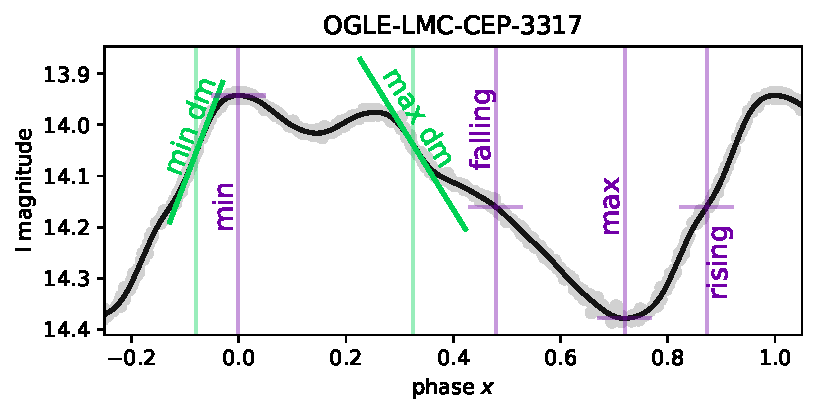
\includegraphics[width=\textwidth]{fig/features.pdf}
        \vspace{-6.8mm}
        \captionof{figure}{Fundamental mode Cepheid fitted to 11th order, with features marked.} 
        \label{fig:features}
    \end{center}
\end{posterbox}



\begin{posterbox}[name=features,column=1,span=2,row=0]{Features \hspace{5.9cm} Clustering}
\begin{multicols}{2}
    In order to describe the general form of the light curve $\{x_i,m_i\}$, we propose as features:
    \begin{description}
        \item[\texttt{x} \texttt{max}, \texttt{x} \texttt{min}:] phases on the extrema. 
        \item[\texttt{K} \texttt{x} \texttt{max}, \texttt{K} \texttt{x} \texttt{min}:] curvatures on the extrema.
        \item[\texttt{dm} \texttt{max}, \texttt{dm} \texttt{min}:] extrema of the derivative,
        \begin{description}
            \item[\texttt{x} \texttt{dm} \texttt{max}, \texttt{dm} \texttt{x} \texttt{min}:] and their phases.
        \end{description}
        \item[\texttt{x} \texttt{falling}, \texttt{x} \texttt{rising}:] midpoint crosses.
        \item[\texttt{P}:] pulsation period, in days.
        \item[\texttt{A}:] pulsation amplitude, in magnitudes.
    \end{description}
    The fit ephemeris (\alert{\texttt{x min}}) was subtracted from all the other phases, and \alert{\texttt{K x min}} was rejected after examination. This left us with 10 features, which are exemplified in Figure \ref{fig:features}. After that, the phases were scaled with $\text{arctanh}\left(2x-1\right)$, and the other features with $\log_{10}$. \vspace{-4mm}
\vfill\null
\columnbreak
    The HDBSCAN* algorithm \citep{Campello2013} was used to cluster the data, using the Python implementation by \cite{McInnes2017}. 

    We used the Chebyshev metric, defined on the feature space as $d_{\infty}(\vec{x},\vec{y})=\max_k(|x_k-y_k|)$, because it gave us 67\% of selection ratio and captured the desired detail on the clusters.

    The selected values for the hyperparameters were \texttt{min\_cluster\_size=5} and \texttt{min\_samples=4}.   This generated more clusters than expected, but with the hybrid algorithm of \cite{Malzer2020}, using $\epsilon=0.047$, the nearest clusters were merged, leaving us with 63 classes and 29\% of rejected data.
\end{multicols}
\end{posterbox}



\begin{posterbox}[name=ident,column=1,below=features,height=bottom]{Identification on the PL diagram}
    We examined the resulting clusters in the PL diagram (Figure \ref{fig:PL}). The largest three seemed to cover the most part of the F, 1O and WVir classes. There were many small clusters on the upper and lower parts of the linear tendencies on the PL diagrams, which were aggregated with the bigger classes. 

    As can be seen on Figure \ref{fig:confusion}, all of the OCVS classes were present, but due to their size differences, the classical 2O and the a1O are only marginally identified.

    \begin{center}
    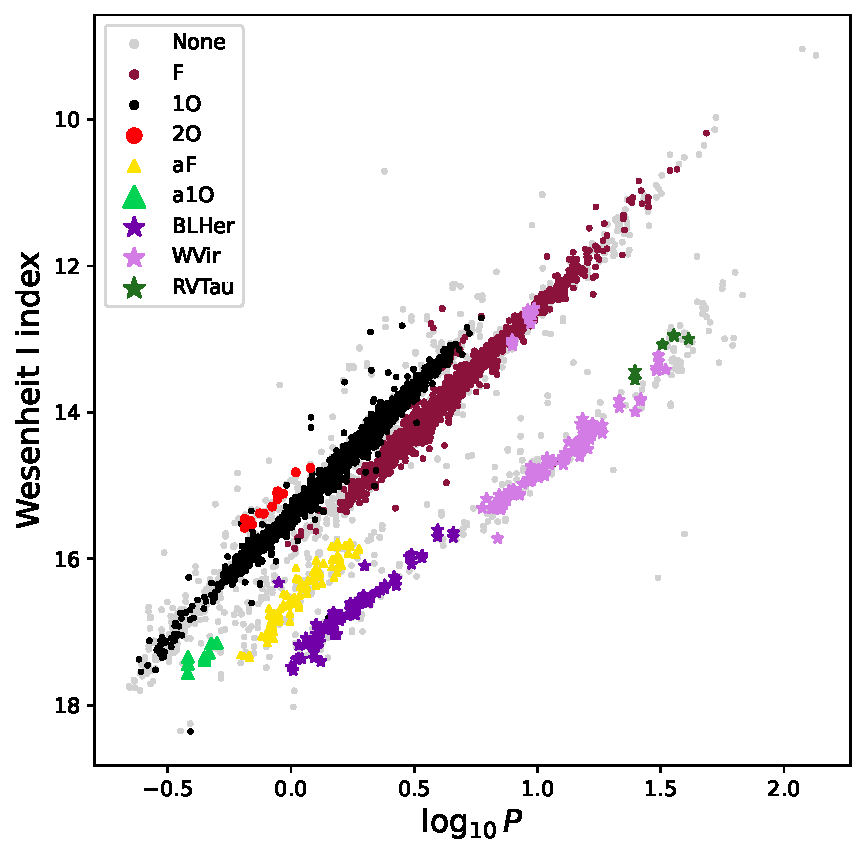
\includegraphics[width=\textwidth]{fig/PL.pdf}
    \vspace{-5.3mm}
    \captionof{figure}{
        PL relation of the LMC Cepheids with the aggregated cluster labels. Here the Wesenheit index is defined as $W=I-1.55(V-I)$.
    }
    \label{fig:PL}
    \end{center}

    \begin{center}
    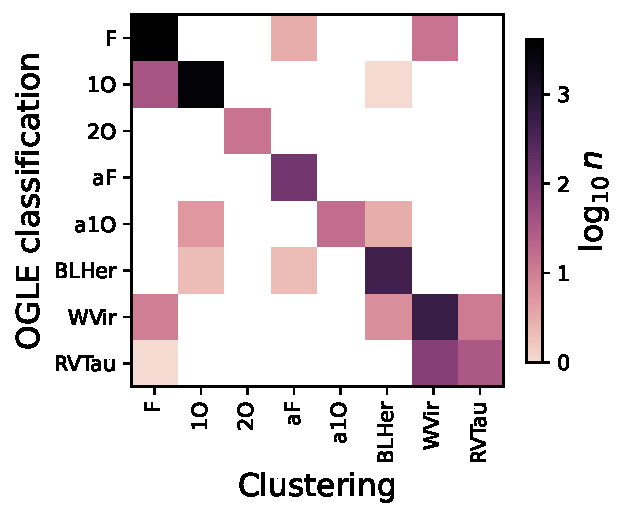
\includegraphics[width=0.9\textwidth]{fig/confusion.pdf}
    \vspace{-3mm}
    \captionof{figure}{
        Confusion matrix between cluster identification and OCVS labels. $n$ is the amount of data in each cell.% The color represents the base 10 log of the amount of data in each cell.
    }
    \label{fig:confusion}
    \end{center}
\end{posterbox}



\begin{posterbox}[name=struct,column=2,below=features]{Hidden morphology of Cepheids}
    Additional to the PL relations, some structure was found on the F, 1O and aF classes as can be seen in Figure \ref{fig:struct}. 
    %This was confirmed in the condensed tree dendogram.

    \vspace{-2mm}
    \begin{center}
    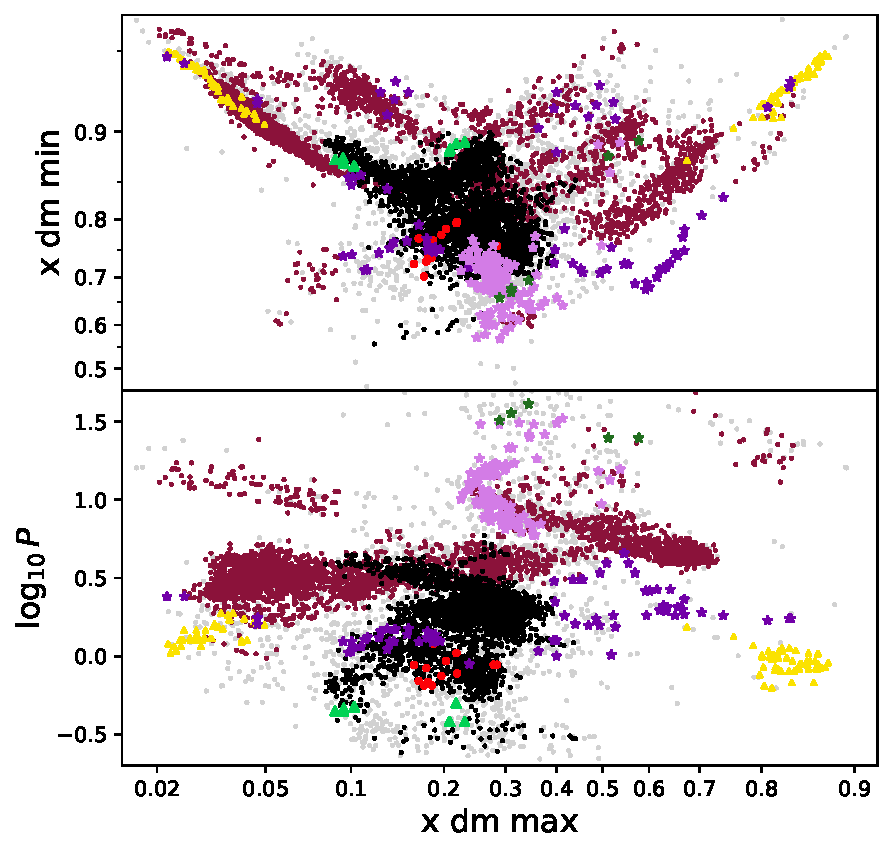
\includegraphics[width=0.93\textwidth]{fig/sctruct.pdf}
    \vspace{-2mm}
    \captionof{figure}{Selection of pair plots from the clustering features. Same legend as in Figure \ref{fig:PL}.}
    \label{fig:struct}
    \end{center}
    \vspace{-2mm}

    It remains to be seen if this structure is related to the Hertzprung progression, as the presence of a bump in the curve could affect the derivative values.
\end{posterbox}



\begin{posterbox}[name=conclusions,column=2,below=struct]{Conclusions and acknowledgments}
    The proposed set of light curve features proved capable of determining the pulsation mode of classical Cepheids, and are able to discern them from the anomalous and type II Cepheids.    
    The presence of Cepheids with a secondary bump reaching beyond the real amplitude compromises some of the features, and it will be explored in the future. 
    
    The authors acknowledge Universidad de los Andes for the grants and computational resources used in this project.
\end{posterbox}


\begin{posterbox}[column=2,below=conclusions,height=bottom]{References}
\tiny
\setlength{\parskip}{0em}
\setlength{\bibsep}{0pt plus 0.8ex}
    \bibliographystyle{aa_url} % style aa.bst
    \bibliography{poster.bib}
\end{posterbox}



\end{poster}
\end{document}




















































